\section{Service Flexibility Agreement}
\label{sec:sfa}

In this section, we introduce the notion of Service Flexibility Agreement (SFA). 
%Cloud Computing provides highly flexible infrastructures in which resources and software services are provisioned on demand through the concept of elasticity.

In current PaaS architectures, the framework grants a certain flexibility to applications.
For example, an application can ask the PaaS framework to spawn more or less VMs according to its needs.
However, the flexibility is entirely controlled by the application.
The intuition behind SFA is to delegate some of the flexibility control to the PaaS framework while still guaranteeing the end user satisfaction.

%Cloud computing provides/supports three different concepts Elasticity, Variable Workload, Scalability  ... the intersection of these concepts is the main power of cloud that can be exploited for energy efficiency and energy optimization purposes within cloud infrastructures.

%Variable Workload %Elasticity
%variable workload, i.e. workloads performance varies over time, elasticity is the appropriate vehicle to enact variable workload in the cloud.

%Scalability
%On the other hand, cloud computing provides scalability both for application, and infrastructure. Therefore, cloud provides a dual solution for application and infrastructure growth.


%We define an application SFA at a fine-grade level of details to model application performance flexibility.
 
%A vehicle for energy optimization
PaaS can exploit automated application scalability in cloud and SFA to optimize energy consumption of applications as a whole within a cloud system.

\begin{figure}[h]
\centering
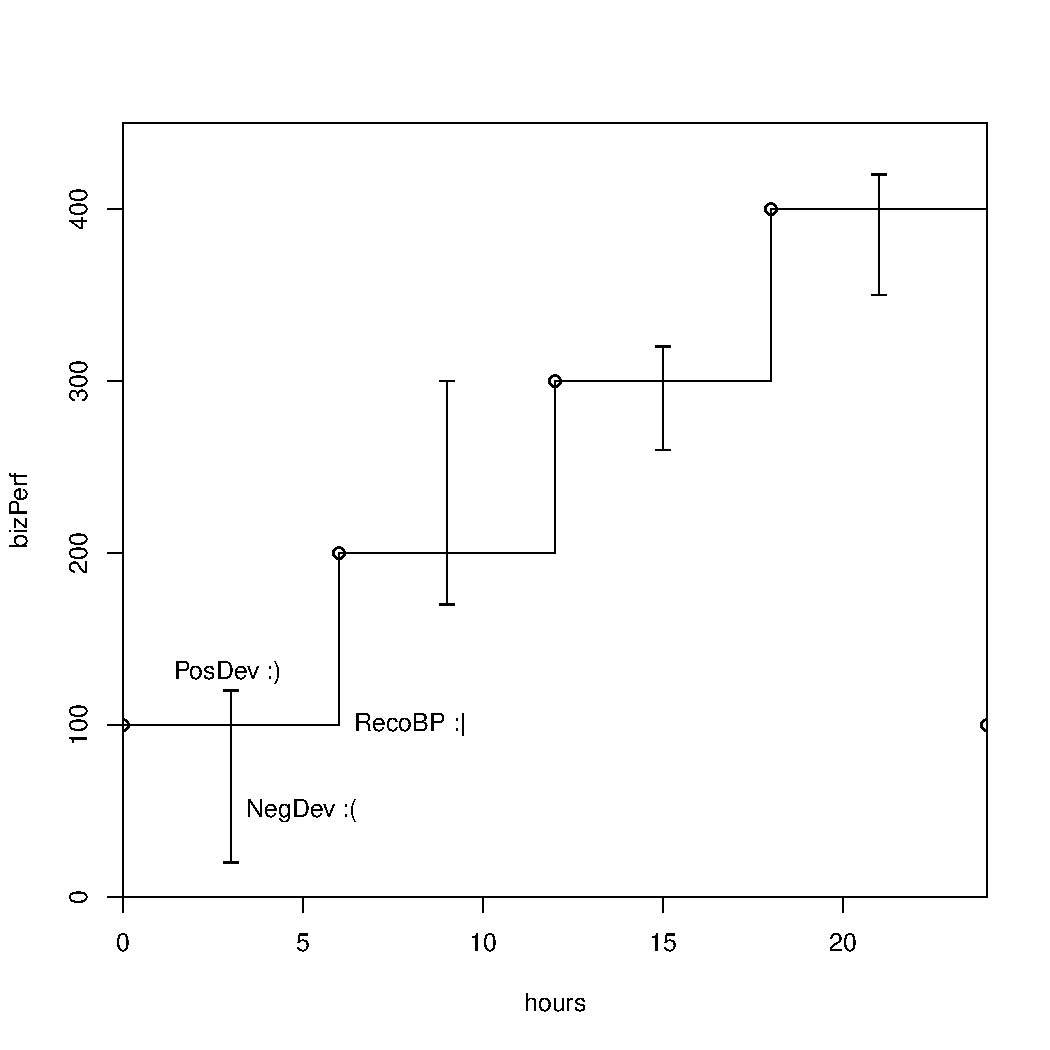
\includegraphics[width=0.99\linewidth]{generated/SFA-candles.pdf}
\caption{Service Flexibility Agreement representation}
\label{fig:EASC}
\end{figure}

An example of SFA is as the following:
\ms{I think you may provide a complete name for variables e.g. RecoBP=Recommended Business Performance, etc.}
\begin{listing}[ht]
\begin{minted} [frame=single, linenos]{yaml}
- Start: 00:00
  End: 06:00
  RecoBP: 100 Hz
  PosDev: 100 Hz/H
  NegDev: 50 Hz/H
- Start: 07:00
  End: 12:00
  RecoBP: 300 Hz
  PosDev: 50 Hz/H
  NegDev: 200 Hz/H
\end{minted}
\caption{SFA example}
\label{lst:SFA}
\end{listing}
%    greenPoints: 1
%    greenPoints: 0
\begin{listing}[ht]
\begin{minted} [frame=single, linenos]{yaml}
- WMName: WM1
    actuator: 'cf scale myApp -i 3'
    defaultPower: '300 W'
    maxBusinessPerf: '100 Page/min'
- WMName: WM2
    actuator: 'cf scale myApp -i 5'
    defaultPower: '500 W'
    maxBusinessPerf: '150 Page/min'
\end{minted}
\caption{Working Modes example}
\label{lst:WMs}
\end{listing}

With respect to a traditional SLA, the SFA adds a few new dimensions: the possibility for the required resources to vary in time, plus the possibility to qualify violations of the required performance.
As shown in listing~\ref{lst:SFA}, for each time frame the SFA defines a recommended business performance. 
The business performance is one of the KPIs of the application.
For example, for a Web server it is the number of pages served per minutes, for a video transcoding service it will be how much gigabit of video transcoded.
In practice, the business performance is expressed in terms of Hertz: that is a number of items processed per unit of time.
We then define a concept called the "Happy points", noted "H".
This is an abstraction of the end-user satisfaction.
An application having zero Happy points means that the end user is reasonably satisfied.
That corresponds to the traditional SLA threshold.
Positive Happy points correspond to "fairly satisfied" (1H) up to "very satisfied" (10H).
Negative Happy points correspond to "fairly unsatisfied" (-1H) up to "very unsatisfied" (-10H).

\ms{We may refer to a function name like HappyPoints that as input receives performance, and as output gives the number of happy points}

We further define the Working Modes (WM) of an application, as shown in listing~\ref{lst:WMs}.
A Working Mode corresponds to the level of performance/resource usage for an application.
In practice, this corresponds to a number of VMs or application instances in terms of containers.
This further corresponds to an average power consumption and an expected business performance. 
Using the SFA, it is now possible to compute the number of Happy points provided by each WM.

%\ms{I believe more concrete definition is required. We need to establish a better relationship between working mode and SFA. We need better describe working mode and to remove green points.}

%\ms{Or we don't need to refer/define working mode. SFA already corresponds to working mode concept, that is SFA provides various performance levels with different power consumptions}

